\documentclass{sig-alternative}
% \documentclass[conference]{IEEEtran}
\usepackage{multirow}
\usepackage{color}
\usepackage{graphics} 
\usepackage{cite}
\usepackage{rotating}
\usepackage{eqparbox}
\usepackage{graphics}
\usepackage{colortbl} 
\usepackage{balance}
\usepackage{picture}
\usepackage{algorithm}
\usepackage{algorithmicx}
\usepackage{algpseudocode}
\renewcommand{\footnotesize}{\scriptsize}
\definecolor{lightgray}{gray}{0.8}
\definecolor{darkgray}{gray}{0.6}
\renewcommand{\algorithmicrequire}{\textbf{Input:}}
\renewcommand{\algorithmicensure}{\textbf{Output:}}
%%% graph
\newcommand{\crule}[3][darkgray]{\textcolor{#1}{\rule{#2}{#3}}}
%\newcommand{\rone}{\crule{1mm}{1.95mm}}
%\newcommand{\rtwo}{\crule{1mm}{1.95mm}\hspace{0.3pt}\crule{1mm}{1.95mm}}
%\newcommand{\rthree}{\crule{1mm}{1.95mm}\hspace{0.3pt}\crule{1mm}{1.95mm}\hspace{0.3pt}\crule{1mm}{1.95mm}}
%\newcommand{\rfour}{\crule{1mm}{1.95mm}\hspace{0.3pt}\crule{1mm}{1.95mm}\hspace{0.3pt}\crule{1mm}{1.95mm}\hspace{0.3pt}\crule{1mm}{1.95mm}} 
%\newcommand{\rfive}{\crule{1mm}{1.95mm}\hspace{0.3pt}\crule{1mm}{1.95mm}\hspace{0.3pt}\crule{1mm}{1.95mm}\hspace{0.3pt}\crule{1mm}{1.95mm}}
\newcommand{\quart}[3]{\begin{picture}(100,6)%1
{\color{black}\put(#3,3){\circle*{4}}\put(#1,3){\line(1,0){#2}}}\end{picture}}
\definecolor{Gray}{gray}{0.95}
\definecolor{LightGray}{gray}{0.975}
% \newcommand{\rone}{}
% \newcommand{\rtwo}{}
% \newcommand{\rthree}{}
% \newcommand{\rfour}{} 
% \newcommand{\rfive}{}
\newcommand{\wei}[1]{\textcolor{red}{Wei: #1}} 

%% timm tricks
\newcommand{\bi}{\begin{itemize}[leftmargin=0.4cm]}
\newcommand{\ei}{\end{itemize}}
\newcommand{\be}{\begin{enumerate}}
\newcommand{\ee}{\end{enumerate}}
\newcommand{\tion}[1]{\S\ref{sect:#1}}
\newcommand{\fig}[1]{Figure~\ref{fig:#1}}
\newcommand{\eq}[1]{Equation~\ref{eq:#1}}

%% space saving measures

\usepackage[shortlabels]{enumitem}  
\usepackage{url}
% \def\baselinestretch{1}


% \setlist{nosep}
%  \usepackage[font={small}]{caption, subfig}
% \setlength{\abovecaptionskip}{1ex}
%  \setlength{\belowcaptionskip}{1ex}

%  \setlength{\floatsep}{1ex}
%  \setlength{\textfloatsep}{1ex}
%  \newcommand{\subparagraph}{}

% \usepackage[compact,small]{titlesec}
% \DeclareMathSizes{7}{7}{7}{7} 
% \setlength{\columnsep}{7mm}

\begin{document}
% \conferenceinfo{FSE}{'15 Bergamo, Italy}
\title{ Analytics Without  Tuning Considered Harmful?}
% \numberofauthors{1}
\author{\alignauthor Wei Fu, Tim Menzies, Xipeng Shen \\
       \affaddr{Computer Science, North Carolina State University, Raleigh, USA}\\
       fuwei.ee, tim.menzies, xipengshen@gmail.com}
\maketitle 
\thispagestyle{plain}
\pagestyle{plain}
\begin{abstract}
One of the ``black arts'' of data mining is setting the tuning
parameters that control  the miner.  We offer a simple,
automatic, and very effective  method for finding those tunings.
For the purposes of learning
software defect predictors this  method can quickly
find  good tunings that  dramatically change   the performance of a learner.
For example,
in this paper we show   tunings that  alter detection  precision  
 from 2\% to 98\%.

These results prompt for a change to standard methods in software analytics.
At least for defect prediction, 
it is no longer enough to just run a data miner and present the result
{\em without}  conducting a tuning optimization study.
The implication for other kinds of  analytics is now  an open and pressing issue.

%RQ1: Does tuning affect learners' performance?
%RQ2: How to choose 

\end{abstract}

% A category with the (minimum) three required fields
\vspace{1mm}
\noindent
{\bf Categories/Subject Descriptors:} 
D.2.8 [Software Engineering]: Product metrics;
I.2.6 [Artificial Intelligence]: Induction

 
\vspace{1mm}
\noindent
{\bf Keywords:} defect prediction, CART, random forests,
differential evolution,
search-based software engineering.

\pagenumbering{arabic} %XXX delete before submission
 
 
\section{Introduction}
 
In the $21^{st}$ century, it is now impossible
to manually browse all the available software project
data. The PROMISE repository of SE data has grown to 200+ projects~\cite{promise15}
and this is just one of over a dozen open-source repositories
that are readily available to researchers~\cite{rod12}.
For example, at the time of this writing (May  2015), our web searches show that Mozilla Firefox has over 1.1 million bug reports, and platforms such as GitHub host over 14 million projects. 

Faced with this information overload,
researchers in empirical SE
use  data miners  to generate 
{\em defect predictors from static code measures}.
Such   measures can be
automatically extracted from the code base, with very little effort
even for very large software systems~\cite{nagappan05}. 

One of the ``black arts'' of data mining is setting the tuning
parameters that control  the choices within a data miner.
Prior to this work, our intuition was that tuning would change the behavior or a data miner, to some degree. Nevertheless, we rarely tuned our  defect predictors 
since we reasoned
that a data miner's default tunings have been well-explored by the developers of those algorithms (in which case
tuning would not lead to large performance improvements).
Also, we suspected that
tuning would take so long and be so CPU intensive that the benefits gained   would not be worth effort.

The results of this paper show that neither of these points is supportable, at least when learning
defect detectors from static code attributes since:
\be
\item
Tuning  defect predictors is {\em remarkably simple};
\item
And can {\em dramatically improve the performance}. 
\ee
More specifically,
this paper explores six research questions about tuning defect predictors for
static code measures:
\bi
\item RQ1: {\em Does   tuning    improve the performance scores of a predictor?} We will show below
 examples of truly dramatic improvement;
e.g.  precision changes from 2\% to 98\%.
\item RQ2: {\em Does tuning change conclusions on what learners are better than others?} 
Numerous recent SE papers (e.g. \cite{lessmann2008benchmarking,hall11,me07b}) claim that some learners are better than others. We show that at least
some of those conclusions are completely changed by tuning.
\item RQ3: {\em Does tuning change conclusions about what factors are most important in software engineering?} Numerous recent SE papers (e.g. ~\cite{bell2013limited,rahman2013how,me02k,moser2008comparative,zimmermann2007predicting,%
herzig2013predicting}) use data miners to conclude that {\em this}
is more important than {\em that} for (e.g.) reducing software project defects.
Given the  tuning results of this paper, we show that such conclusions need to be revisited.
\item  RQ4: {\em Is tuning easy?} We show that one of the simpler multi-objective optimizers
(differential evolution~\cite{storn1997differential}) works very well for tuning defect predictors. 
\item RQ5: {\em Is tuning impractically slow?}. We achieved dramatic improvements in the performance scores
of our data miners in less than 100 evaluations (!!); i.e. very
quickly.
\item RQ6: {\em Should data miners be used ``off-the-shelf'' with their default tunings?} 
At least for defect prediction from static code measures, our answer is an emphatic ``no'' (and
the implication for other kinds of software analytics is now an open and urgent question).
\ei
Before beginning, we digress for one  clarification.
This paper is {\em not} arguing that
software analytics is somehow wrong-headed or misguided.
In the age of the Internet and global access to software engineering data,
there exists the  problem of information overload. {\em Something} must be done to
allow analysts to make conclusions via an automatic analysis over a lot of data.
The results of this paper is that for a particular local context
(a specific data set and a specific goal) there exists  
methods for optimizing the conclusions reached in that context.  
Those conclusions
may not generalize to other contexts but this  is not a council for despair. 
As shown here, 
there  exists general methods for finding
local conclusions in a particular context. Further,
those
methods are  very simple to implement and very fast to execute.


\section{But is This a New Result?}


In  other fields, the impact of tuning is well understood. However, as we argue
in this section, this result is not properly  acknowledged  in the field of software analytics. 

The formal definitions of data mining stresses that these learners are heuristic explorers
of a truly   vast space of the possible models within a data set~\cite{mitchell1982generalization}. For example, given 20 columns of boolean variables,
there are $2^{20}$ possible models. Data mining is practical since various heuristics
allow automatic algorithms to ignore most of those possibilities. 

While that heuristic search makes data mining possible, it also means that tunings
can significantly affect what comes out of a data miner.
When we tune a data miner, what we are really doing is changing how a learner applies
its heuristics. This means tuned data miners use different heuristics, which means they ignore different possible models, which means they return different models.     

The fact that {\em how} we learn changes {\em what} we learn is not acknowledged
in the field of software analytics.
There exists many research papers
that use data miners to   show that certain factors
are more influential than others for (say)
predicting defects. As shown below, such conclusions can be dramatically
changed by the tuning process since those  ``influential'' factors are very different pre- and post- tuning. Also, those factors tend to  change from project to project or if the goal
of the tuning is altered.
Hence, many old papers    need to be revisited  and perhaps revised~\cite{bell2013limited,rahman2013how,me02k,moser2008comparative,zimmermann2007predicting,herzig2013predicting}.  
For example, one of us (Menzies) used data miners
to assert that some factors were more important than others for predicting
successful software reuse~\cite{me02k}. That assertion should now be doubted since that
Menzies did not conduct a tuning study before reporting what factors the data miners
found were most influential.

Further, several  prominent IEEE TSE papers~\cite{lessmann2008benchmarking,hall11,me07b} have claimed 
that learnerX is better than learnerY for some software analytics task.
For example, a recent IEEE TSE article claimed that the 
CART decision tree learner was far worse than Random Forests for
software defect prediction~\cite{lessmann2008benchmarking}. 
Such conclusions do not survive tuning.
For example,
after tuning, the worst learner (CART) can perform just as well as the supposedly
best learner (Random Forest). Hence, all those prior results that ranked learners for software
analytics now need to be revisited (and perhaps revised).

Thirdly, it is a standard practice to use the default ``off-the-shelf'' tunings  for data mining tools (previously
we have defended that approach, arguing that it
encourages reproducibility~\cite{me15:book1}). That ``off-the-shelf''  policy
can no longer be condoned. For example, suppose our default
number of trees in  a Random Forest was   $F=100$ (which is the default in our implementation).
After tuning, we see that our optimizer often uses $F$ values that are nowhere near that default:

% {\scriptsize
% \[F \in \left\{\begin{array}{l} 55,  65, 70,   82, 88, 96, 100,  102,  104, 107,\\
%                                 108,  119, 133,  140, 140,   147,  145,  142   \end{array}\right\}
% \]}


% {\scriptsize
% \[F \in \left\{\begin{array}{l} 50, 59, 63, 63, 69, 71, 81, 85,85, 88,\\
%                                 92, 95, 96, 99, 99,  100, 104, 106, 107,\\
%                                 109, 111, 112, 121, 121, 123, 125, 128,\\
%                                 131, 132, 135, 140, 141, 141, 150   \end{array}\right\}
% \]}



{\scriptsize
\[F \in \left\{\begin{array}{l} 50, 58, 59, 63, 63, 66, 67, 73, 74, 74, \\
                                75, 77, 80, 82, 85, 96, 96, 97, 97, 101, \\
                                103, 107, 111, 111, 112, 120, 125, 125,  \\
                                130,130, 138, 144, 149, 150   \end{array}\right\}
\]}

\begin{figure*}[t]
\renewcommand{\baselinestretch}{0.8}\begin{center}
{\scriptsize
\begin{tabular}{c|l|p{4.7in}}
amc & average method complexity & e.g. number of JAVA byte codes\\\hline
avg\_cc & average McCabe & average McCabe's cyclomatic complexity seen
in class\\\hline
ca & afferent couplings & how many other classes use the specific
class. \\\hline
cam & cohesion amongst classes & summation of number of different
types of method parameters in every method divided by a multiplication
of number of different method parameter types in whole class and
number of methods. \\\hline
cbm &coupling between methods &  total number of new/redefined methods
to which all the inherited methods are coupled\\\hline
cbo & coupling between objects & increased when the methods of one
class access services of another.\\\hline
ce & efferent couplings & how many other classes is used by the
specific class. \\\hline
dam & data access & ratio of the number of private (protected)
attributes to the total number of attributes\\\hline
dit & depth of inheritance tree &\\\hline
ic & inheritance coupling &  number of parent classes to which a given
class is coupled (includes counts of methods and variables inherited)
\\\hline
lcom & lack of cohesion in methods &number of pairs of methods that do
not share a reference to an instance variable.\\\hline
locm3 & another lack of cohesion measure & if $m,a$ are  the number of
$methods,attributes$
in a class number and $\mu(a)$  is the number of methods accessing an
attribute, 
then
$lcom3=((\frac{1}{a} \sum_j^a \mu(a_j)) - m)/ (1-m)$.
\\\hline
loc & lines of code &\\\hline
max\_cc & maximum McCabe & maximum McCabe's cyclomatic complexity seen
in class\\\hline
mfa & functional abstraction & number of methods inherited by a class
plus number of methods accessible by member methods of the
class\\\hline
moa &  aggregation &  count of the number of data declarations (class
fields) whose types are user defined classes\\\hline
noc &  number of children &\\\hline
npm & number of public methods & \\\hline
rfc & response for a class &number of  methods invoked in response to
a message to the object.\\\hline
wmc & weighted methods per class &\\\hline
\rowcolor{lightgray}
defect & defect & Boolean: where defects found in post-release bug-tracking systems.
\end{tabular}
}
\end{center}
\caption{OO measures used in our defect data sets.}\label{fig:ck}
\end{figure*}




The  good news of this paper  is that {\em tuning is very easy}.
This result is both novel and unexpected.
A standard run of such evolutionary optimizers requires   thousands,
if not millions, of evaluations. However, in a result that we found startling, that  differential evolution can find useful settings for learners generating defect predictors
in less than 100 evaluations (i.e. very quickly).
Hence,   the ``problem'' (that
tuning changes the conclusions) is really
an exciting opportunity. At least for defect prediction,
 learners are very   amenable to tuning. Hence, 
 they are  also very
amenable to significant performance improvements. Given the low
number of evaluations required, then we assert that tuning
  should be standard practice
for anyone building defect predictors.

That said, the bad news is that, for defect
prediction, tuning results in dramatic changes in
  what is learned from that data. Therefore, it is now an open and pressing research issue to check if
analytics without parameter tuning is considered {\em harmful} or, at the 
very least, {\em misleading}.
Clearly, we  must now revisit all prior results   based on
``off-the-shelf'' tunings.
Further,
it is no longer enough to just run a data miner and report the result
{\em without} first conducting an tuning optimizations study.

% \section{Motivating Example}\label{sect:eg}

% This section is  a  demonstration
% of the impact of tuning.
 
% Suppose  a researcher wants to use linear regression
% to test if Halstead's~\cite{halstead77} measures
% of   function complexity
% (number of symbols programmers has to understand) are   {\em better than}
% mere lines of code for predicting
% software defects.  That researcher might believe that Halstead's cognitive approach to
% software bugs is better suited to code refactoring tools since it offers 
% more ways to alter functions that just some coarse grain lines of code measure.


% To test that belief, our  researcher applies regression to  some defect logs.
%  Here are two equations (learned from the NASA data at goo.gl/pGDfvp)
% that use just lines of code or the Halstead measures $N,V,L,D,I,E,B,T$ seen in a
% software module (in this case, a  function).
% Note that the Halstead correlation $c_2$
% is worse than the $c_1$ correlation  from lines of code-- which suggests
%  our researcher should not use Halstead .

% {\scriptsize \[
% \begin{array}{l|l|ll}
% \mathit{measures} & d= \mathit{\#defects} & \mathit{correlation}\\\hline
% \mathit{LOC}   &d_1= 0.0164 +0.0114\mathit{LOC}\ & c_1 = 0.65\\\hline
% \mathit{Halstead} & d_2= 0.231 + 0.00344N  +  0.0009V    \\    
%                  &   - 0.185L- 0.0343D      - 0.00541I  \\ 
%                  & + 0.000019E + 0.711B  - 0.00047T  & c_2=-0.36  
% \end{array}
% \]
% }
 

% \noindent
% We now explore how tuning can change the above  conclusion. Suppose the  predictors $d_1$ and $d_2$  learned from LOC or Halstead
% are used to call an inspection
% team to check for errors in   parts of the code using:
% \begin{equation}\label{eq:yesno}\scriptsize
% \mathit{inspect}= \left\{
% \begin{array}{ll}
% d_i \ge T \rightarrow \mathit{Yes}\\
% d_i <   T \rightarrow \mathit{No} 
% \end{array}\right.
% \end{equation}
% \fig{pd1} shows the effects of tuning. Not surprisingly,
% at $T=0$, all modules get inspected so the false alarm rate is very high. To reduce that
% problem, we can increase $T$:   the false alarm rate falls below
% 20\% at $T=0.45$ (for Halstead). 

 

% \begin{figure}[!t] 

% \renewcommand{\baselinestretch}{0.8}
% {\scriptsize
% \begin{center}

% \% recall (probability of detection):   

% 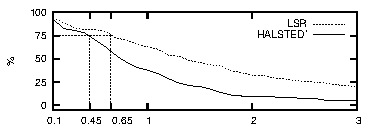
\includegraphics[width=3in]{lsrvscostpd.pdf}

% \% false alarms:

% 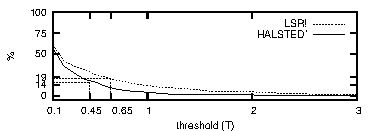
\includegraphics[width=3in]{lsrvscostpf.pdf}
% \end{center}}
% \caption{
%  Y-axis shows probability of false alarm,
%   and
%   probability of recognizing defective modules  seen using \mbox{$d_i \ge T$}.
%   Curves calculated from the KC2 dataset from the PROMISE repository goo.gl/pGDfvp.
%  }\label{fig:pd1}
%  \end{figure}
 
% Note that either the Halstead or LOC detector can reach some desired
% level of recall, regardless of their correlations, just by
% selecting the appropriate threshold value. For example, in \fig{pd1}, see the recall=75\% values
% found at {\em either} $d_i\ge 0.65$ or $d_2\ge 0.45$ (and at the threshold, the false alarm rates
% were very similar: 14\% and 19\%).

% The  point here is that   the true value of a detector
% could not be assessed {\em without} conducting a  tuning study in the context of some business case (in this case, 
% issuing a request to an inspection team to review some module).  
% Hence, it is important to explore tuning.

% The rest of this paper repeats the analysis of this section, but for 
% more complex learners.

\section{Background Notes}
 

\subsection{Defect Prediction}


This section is our standard introduction to defect prediction~\cite{me15:book1},
plus    some new results from Rahman et al.~\cite{rahman14:icse}. 
 




Human programmers are clever, but flawed. Coding  adds functionality, but also defects.
Hence, software sometimes crashes (perhaps at the most awkward or dangerous moment) or delivers
the wrong functionality. For a very long list of software-related errors,
see  Peter Neumann's ``Risk Digest'' at catless.ncl.ac.uk/Risks.

Since programming inherently
introduces defects into  programs, is important to thoroughly {\em test} software before it is {\em used}.
Such testing  can be very expensive.
Software assessment budgets are finite
while assessment effectiveness increases 
exponentially with assessment effort.
Lowry et al. warn that  
the state space explosion problem imposes
strict limits on how much a system can be explored
via automatic formal methods~\cite{lowrey98}.
For standard black-box testing methods,
a {\em linear} increase
in the confidence $C$ that we have found all defects
can take {\em exponentially} more effort.
For example, for one-in-a-thousand detects,
moving $C$ from  
90\% to 98\% nearly doubles the number of  tests (2301 to   3910 black box
probes, respectively)\footnote{A randomly selected 
input to a program will find a fault with probability $p$.
After $N$ random black-box tests, the chances of the inputs 
not revealing any fault 
is $(1-p)^N$. Hence, the chances $C$ of seeing the fault is $1-(1-p)^N$
which can be rearranged to 
 $N(C,p)=log(1 -
C)/log(1-p)$. For example, $N(0.90,10^{-3})=2301$.}.

Exponential costs quickly exhaust finite resources.
Standard practice is to apply the best
available assessment methods on the sections of the program that the
best available domain knowledge declares is most critical.  We endorse
this approach.  Clearly, the most critical sections require the best
known assessment methods. However, this focus on certain sections
can blind us to defects in other areas.
Therefore, standard practice should be augmented
with a  {\em
lightweight sampling policy} to explore the rest of the system.  This
sampling policy will always be incomplete.
Nevertheless, it is the recommended option when
resources do not permit a complete assessment of the whole system.

One such lightweight sampling policy is defect predictors learned from static code attributes.
Given software described using (for example) the attributes of \fig{ck}, it is possible
to use standard data mining technology to learn where the probability of software defects is highest.
Such defect predictors learned from
static code attributes are   {\em easy to
use}, {\em widely-used}, and {\em useful} to use.

{\em Easy to use:} Static code attributes can be automatically collected, even for very large systems~\cite{nagappan05}.
Other methods, like  manual code reviews, are far slower and far more labor-intensive.
For example, depending on the review methods, 8 to 20 LOC/minute can be
inspected and this effort repeats for all members of the review team,
which can be as large as four or six people~\cite{me02f}. 

%%%%%%%%%%%%%%%% list of parameters%%%%%%%%%%%%%%%%%%%%%
\renewcommand\arraystretch{1.2}
\begin{figure*}[t!]
\scriptsize
  \centering
	\begin{tabular}{|c|c|c|c|l|}
	\cline{1-5}
	\begin{tabular}[c]{@{}c@{}}Learner \\ Name\end{tabular} & Parameters & Default &\begin{tabular}[c]{@{}c@{}}Tuning\\ Range\end{tabular}& 
\multicolumn{1}{c|}{Description} \\ \hline
	\multirow{8}{*}{\begin{tabular}[c]{@{}c@{}}Where-based\\ Learner\end{tabular}} 
	& threshold & 0.5 &[0.01,1]& The value to determine defective or not .\\ \cline{2-5} 
	& infoPrune & 0.33 &[0.01,1]& The percentage of features to consider  for the best 
split to build CART tree\footnote{Since the Where-based learner will build two trees, the first 
one is for clustering and the second one is building prediction model. we explicitly call Where-
clustering tree and CART tree, respectively}. \\ \cline{2-5} 
	 & min\_sample\_split & 4& [1,10]& The minimum number of samples required to split an internal node of
CART tree. \\ \cline{2-5} 
	 & min\_Size & 0.5 &[0.01,1]& \begin{tabular}[c]{@{}l@{}}Finds min\_sample 
in Where-clustering trees  using  ${n\_samples}^ {min\_Size}$.
\end{tabular} \\ \cline{2-5} 
    & wriggle & 0.2 &[0.01, 1] & The threshold to determine which branch in  Where tree to be pruned\\ \cline{2-5}
	 & depthMin & 2 & [1,6]&The minimum depth of the tree below which no pruning for Where-
clustering tree. \\ \cline{2-5} 
	 & depthMax & 10 &[1,20]& The maximum depth of the Where-clustering tree. \\ \cline{2-5} 
	 & wherePrune & False &T/F& Whether or not to prune the Where-clustering tree. \\ \cline{2-5}
	 & treePrune & True &T/F& Whether or not to prune the classification tree built by CART. \\ \cline{2-5} 
\hline
\multirow{4}{*}{CART} & threshold & 0.5 &[0,1]& The value to determine defective or not. \\ \cline{2-5} 
	 & max\_feature & None &[0.01,1]& The number of features to consider when looking for the best 
split. \\ \cline{2-5} 

	 & min\_sample\_split & 2 &[2,20]& The minimum number of samples required to split an 
internal node. \\ \cline{2-5} 
	 & min\_samples\_leaf & 1 & [1,20]&The minimum number of samples required to be at a leaf 
node. \\ \cline{1-5}  
       \multirow{5}{*}{\begin{tabular}[c]{@{}c@{}}Random \\ Forests\end{tabular}}  & threshold & 0.5 & [0.01,1] & The value to determine defective or not. \\ 
\cline{2-5} 
	 & max\_feature & None &[0.01,1]& The number of features to consider when looking for the best 
split. \\ \cline{2-5} 
	 & max\_leaf\_nodes & None &[1,50]& Grow trees with max\_leaf\_nodes in best-first fashion. \\ \cline{2-5} 
	 & min\_sample\_split & 2 &[2,20]& The minimum number of samples required to split an 
internal node. \\ \cline{2-5} 
	 & min\_samples\_leaf & 1 &[1,20]&The minimum number of samples required to be at a leaf 
node. \\ \cline{2-5} 
	 &  n\_estimators & 100 & [50,150]&The number of trees in the forest.\\ \cline{2-5}
	 \hline

	\end{tabular}
    \caption {List of parameters to be tuned.}
\label{fig:parameters}
\end{figure*}
{\em Widely used:} Many researchers and industrial practitioners  use static attributes to guide software 
quality predictions.
 Defect prediction models have been reported
to have been used at Google~\cite{lewis13}.
Verification and validation (V\&V) textbooks
(\cite{rakitin01}) advise using static code complexity attributes
to decide which modules are worthy of manual inspections.  
For several  years, one of us (Menzies) worked on-site at the NASA software Independent Verification
and Validation facility
and he
knows of several large government software contractors that won't
review software modules {\em unless} tools like McCabe predict that
they are fault prone.  


{\em Useful:}
Defect predictors often  find the location of  70\% (or more)
of the defects in code~\cite{me07b}.
Defect predictors developed at NASA~\cite{me07b} have also been used in software development companies outside the US (in Turkey). When the inspection teams focused on the modules that trigger the defect predictors, they found up to 70\% of the defects using just 40\% of their QA effort (measured in staff hours)~\cite{tosun10}.
A subsequent study on the Turkish software
compared how much code needs to be inspected using
random selection vs. selection via defect
predictors. Using random testing, 87\% of the files
would have to be inspected in order to detect 87\%
of the defects. Further, if the inspection process
was restricted to the 25\% of the files that trigger
the defect predictors, then 88\% of the defects
could be found. That is, the same level of defect
detection (after inspection) can be achieved using
$(87-25)/87=71$\%less effort
\cite{tosun09}.


Defect predicting technology has been
commercialized in many tools including {\it Predictive}~\cite{turner06}, a
 product suite to analyze and predict
defects in software projects. Predictive was observed to
highlight similar issues to those found   with the more expensive tools. Significantly,
Predictive was able to faster process a larger code
base than the more expensive tool~\cite{turner06}.

The success of this method in  predictors in finding bugs is   markedly
higher than other currently-used
industrial
methods such as manual code reviews. For example, 
a  panel at {\em IEEE Metrics
2002}~\cite{shu02} concluded that manual software  reviews can find ${\approx}60\%$ 
of defects.
In other work, 
Raffo documents the typical    defect detection capability of
industrial review methods:   around 50\%
 for full Fagan inspections~\cite{fagan76} to
21\% for less-structured inspections.

Note only do static code defect predictors perform well compared to manual methods,
they also are competititve with certain automatic methods.
At ICSE'14, Rahman et al.~\cite{rahman14:icse} compared:
\bi
\item The static code analysis tools FindBugs, Jlint, and Pmd;
\item Against static code defect predictors
(which they called ``statistical defect prediction'') build using logistic regression.
\ei
They found  no significant differences in the cost-effectiveness
of these  approaches. Given this equivalence, it is significant to note that 
static code defect prediction can be quickly adapted to new languages by building lightweight
parsers that find   information like \fig{ck}. The same is not true for   static code analyzers-- these need  extensive modification before they can be used on new
languages.



 

\subsection{Data Mining Algorithms}
 
There are many ways to build defect predictors
such as  CART~\cite{brieman00}, Random Forest~\cite{breiman84}, 
and WHERE~\cite{menzies2013local}.
For this study, we use the CART and Random Forest  from 
SciKitLearn~\cite{scikit-learn} (and
WHERE is available from
github.com/ai-se/where).
 We use  these algorithms, for the following reasons.
CART and Random Forest were mentioned in
a recent IEEE TSE paper by Lessmann et al.~\cite{lessmann2008benchmarking} that compared 21  
learners for  defect prediction.
That study ranked  CART  worst  and Random Forest as best.
In a demonstration of the impact of tuning,
this paper shows  we can {\em reverse} the conclusions of  Lessmann et al. such that CART
performs just as well as
 Random Forest.
This
 paper also presents results with WHERE-based learner since, as shown below,
it offers an interesting case study on the benefits of tuning.
  

\subsection{Learners and Their Tunings}


Our learners use the tuning parameters of \fig{parameters}. This section describes those parameters.

CART, Random Forest, and WHERE-based learners are all  tree learners that divide a data set, then recurse
on each split.
All these learners
generate numeric predictions which are converted
into binary ``yes/no'' decisions via \eq{yesno}.

\begin{equation}\label{eq:yesno}\scriptsize
\mathit{inspect}= \left\{
\begin{array}{ll}
d_i \ge T \rightarrow \mathit{Yes}\\
d_i <   T \rightarrow \mathit{No} ,
\end{array}\right.
\end{equation}
The splitting process is controlled by numerous tuning parameters.
If data contains more than {\em min\_sample\_split}, then a split is attempted.
On the other hand, if a split contains no more than {\em min\_samples\_leaf}, then recursion stops. CART and Random Forest use a 
user-supplied constant for this parameter while
WHERE-based learner firstly computes this parameter $m$={\em min\_samples\_leaf} from the size of the data
sets via  $m=\mathit{size}^\mathit{min\_size}$ to build an initial  clustering tree.
Note that WHERE builds {\em two} trees: the initial clustering tree (to find similar sets of data)
then a final decision tree (to learn rules that predict for each similar cluster)\footnote{A
frequently asked question is why does WHERE build two trees--
would not   a single tree suffice? The answer is, as shown below,  tuned WHERE's twin-tree approach 
generates very precise predictors.}.
The tuning parameter  {\em min\_sample\_ split } controls the construction of the
final decision tree (so, for WHERE-based learner,
{\em min\_size} and {\em min\_sample\_split} are the parameters to be tuned).

These learners use different techniques to explore the splits:
\bi
\item
CART finds the attributes whose ranges contain rows with least variance in the number
of defects\footnote{If an attribute ranges $r_i$ is found in 
$n_i$ rows each with a  defect count variance of $v_i$, then CART seeks the attributes
whose ranges minimizes $\sum_i \left(\sqrt{v_i}\times n_i/(\sum_i n_i)\right)$.}.
\item
Random Forest    divides data like CART then  builds $F>1$  trees,
each time using some random subset of
the attributes. 
\item
When building the initial cluster tree, WHERE projects the data on to a dimension it synthesizes from the raw data using
a process analogous to principle component analysis\footnote{
PCA  synthesises  new
attributes $e_i, e_2,...$
that extends across the dimension of greatest  variance in the data  with attributes $d$.  
This process  combines
redundant  variables into a smaller set of variables  (so $e \ll d$) since those
redundancies become (approximately) parallel lines
in $e$ space. For all such redundancies \mbox{$i,j \in d$}, we 
can ignore $j$ 
since effects that change over $j$ also
change in the same way over $i$.
PCA is also useful for skipping over noisy variables from $d$-- these
variables are effectively ignored since    they  do not contribute to the variance in the data.}.
WHERE  divides  at the median point of that projection.
On recursion,
this generates the initial clustering tree, the leaves of which are clusters of  very similar examples. After that, when building 
the final decision tree, WHERE pretends its clusters are ``classes'', then 
asks the InfoGain of the
Fayyad-Irani discretizer~\cite{FayIra93Multi}, to rank the attriubutes, where {\em infoPrune} is used.
WHERE's final decision tree generator then ignores everything except the top   {\em infoPrune} percent of the sorted
attributes.
\ei
Some tuning parameters are learner specific:
\bi
\item
{\em Max\_feature} is used by
CART and Random Forest to select the number of attributes
used to build one tree.
CART's default is to use all the attributes while 
Random Forest usually selects the square root of the number
of attributes.
\item
  {\em Max\_leaf\_nodes} is the upper bound on leaf notes generated in a 
  Random Forest.
\item {\em Max\_depth} is the upper bound on the depth of the CART tree.  
 \item
WHERE's initial clustering
tree generation will always split up to {\em depthMin} number of branches.
After that, WHERE will only split data if the mean performance scores of the two halves
is ``trivially small'' (where ``trivially small'' is set by the   {\em wriggle} parameter). 
\item
WHERE's   {\em tree\_prune} setting controls how   
WHERE prunes back superflous parts of the final decision tree. 
If a decision sub-tree and its parent have the same 
majority cluster
(one that occurs most frequently), then if {\em tree\_prune} is enabled, we prune that decision sub-tree.
\ei



\subsection{Tuning Algorithms}


 \subsubsection{Parametric Tuning Algorithms}
The  goal of this paper is to adjust the tuning parameters of \fig{parameters}
in order to   optimize (improve) some particular performance scores
generated by a particular learner being applied to  a particular data set.
For this task, we do not use traditional parametric numeric optimizer  
such as  gradient descent optimizers~\cite{saltelli00} that require models comprised of
differential functions (i.e. functions of real-valued variables whose derivative exists at each point in its domain).
This is impractical  for  our learners since their internal states are   not a smoothly differential continuous function.
Rather, learners being tuned  contain many regions with many different properties (tuning options can
drive the learner into very different modes with very different performance properties).


 \subsubsection{Non-Parametric Tuning Algorithms}
 
Non-parametric  optimizers   make no assumption
about the internal structure of the model.
There are many such optimizers:
\bi
\item
Simulated annealing~\cite{fea02a,me07f};
\item
A wide range of genetic algorithms~\cite{goldberg79} augmented by
techniques such as differential evolution~\cite{storn1997differential}, tabu search and scatter search~\cite{Glover1986563,Beausoleil2006426,Molina05sspmo:a,4455350};
\item
Particle swarm optimization~\cite{pan08}; 
\item 
Numerous ``decomposition approaches'' that uses
    heuristics to decompose the total space into   small problems,   then applies a
    simpler optimizer to each region including \mbox{$\varepsilon$-domination}~\cite{deb05} and MOEA/D ~\cite{zhang07};
    \item 
    Response surface methods~\cite{krall15,Zuluaga:13};
    \item
    And many others as well.
    \ei
From all the above methods, how do we select which optimizers to apply to tuning data miners?
Cohen~\cite{cohen95} advises comparing new 
 methods against the simplest possible alternative. 
Holte~\cite{holte93} recommends using very simple  learners
 as a
kind of ``scout'' for a  preliminary analysis of a data
set (to check if that data really requires a more
complex analysis).

To find our ``scout'',  we used engineering judgement to sort  the above algorithms from simplest to most complex.
Of the optimizers listed above, the simplest are simulated annealing (SA)  and 
differential evolution (DE), each of which can be coded in less than a page of some high-level scripting language. Our reading of the current literature is that there are more  advocates for
differential evolution than
  SA:
  \bi
  \item
  When the MOEA/D community requires a secondary optimizer, they often use  differential evolution~\cite{zhang07,5583335}.
  \item
 Vesterstrom and Thomsen~\cite{Vesterstrom04} found DE to be competitive with 
   particle swarm optimization and other GAs.
   \ei
DEs have been applied before for   parameter tuning (e.g. see~\cite{omran2005differential, chiha2012tuning}) but this is the first time they have been applied to
optimize defect prediction from static code attributes.  
The psuedocode for differential evolution is shown in Algorithm~\ref{alg:DE}.
In the following description, 
    superscript numbers denotes a line in that figure.


\begin{algorithm}[!t]
\caption{Pesudocode for DE with Early Termination}
\label{alg:DE}
\scriptsize
\begin{algorithmic}[1]
\Require $\mathit{np} = 10$, $f=0.75$, $cr=0.3$, $\mathit{life} = 5$, $\mathit{Goal} \in \{\mathit{pd},f,...\}$
\Ensure $S_{best}$

~\\
     
     \Function{DE}{$\mathit{np}$, $f$, $cr$, $\mathit{life}$, $\mathit{Goal}$}
 \State $Population  \gets $ InitializePopulation($\mathit{np}$)   
 \State $S_{best} \gets $GetBestSolution($Population $)
 \While{$\mathit{life} > 0$}
\State $NewGeneration \gets \emptyset$
\For{$i=0 \to \mathit{np}-1$}
\State $S_i \gets$ Extrapolate($Population [i], Population , cr, f$)
\If {Score($S_i$) >Score($Population [i]$)}
\State $NewGeneration$.append($S_i$)
\Else
\State $NewGeneration$.append($Population [i]$)
\EndIf
\EndFor
\State $Population  \gets NewGeneration$
\If{$\neg$ Improve($Population $)}
\State $life -=1$
\EndIf
\State $S_{best} \gets$ GetBestSolution($Population $)
 \EndWhile
\State \Return $S_{best}$
\EndFunction
\Function{Score}{$Candidate$}
   \State set tuned parameters according to $Candidate$
   \State TrainLearner()
   \State $scores \gets$TestLearner()   
   \State \Return$\mathit{Goal}(scores)$  
\EndFunction
\Function{Extrapolate}{$old, pop, cr, f$}
  \State $a, b, c\gets threeOthers(pop,old)$  
  \State $newf \gets \emptyset$
  \For{$i=0 \to \mathit{np}-1$}
       \If{$cr < random()$}
         \State $newf$.append($old[i]$)
                \Else
                  \If{typeof($old[i]$) == bool}
                    \State $newf$.append(not $old[i]$)
         \Else
          \State $newf$.append(trim($i$,($a[i] + f * (b[i] - c[i]$)))) 
         \EndIf
       \EndIf
  \EndFor
 \State \Return $newf$
\EndFunction
        \end{algorithmic}            
\end{algorithm}
 

 \begin{figure*}[!t]

\renewcommand{\baselinestretch}{0.8}
\scriptsize
\centering
  \begin{tabular}{c c c c c c c c c c }\hline
  Dataset &antV0&antV1&antV2&camelV0&camelV1&ivy&jeditV0&jeditV1&jeditV2
\\\hline
  training &20/125 &40/178 &32/293 &13/339 &216/608 &63/111 &90/272 &75/306 &79/312
\\  tuning  &40/178 &32/293 &92/351 &216/608 &145/872 &16/241 &75/306 &79/312 &48/367
\\  testing &32/293 &92/351 &166/745 &145/872 &188/965 &40/352 &79/312 &48/367 &11/492
\\ \hline
  Dataset &log4j&lucene&poiV0&poiV1&synapse&velocity&xercesV0&xercesV1
\\\hline
  training &34/135 &91/195 &141/237 &37/314 &16/157 &147/196 &77/162 &71/440
\\  tuning  &37/109 &144/247 &37/314 &248/385 &60/222 &142/214 &71/440 &69/453
\\  testing &189/205 &203/340 &248/385 &281/442 &86/256 &78/229 &69/453 &437/588
\\  \end{tabular}

   \caption{Data used in this experiment. 
   E.g., the top left data set has 20 defective classes out of 125 total.
   See \tion{dataa} for explanation of {\em training, tuning, testing} sets.
   }\label{fig:data1}
\end{figure*} 

DE is an evolutionary algorithm where the next {\em NewGeneration} is learnt from
a current {\em Population}.  Our DE's lose one ``life''
when e new is no better than  current (terminating when ``life'' is zero)$^{5}$.
Each candidate solution in the {\em Population}  
is a pair of {\em (Tunings, Scores)}.  {\em Tunings} are selected from
\fig{parameters} and {\em Scores} come from training a learner using those parameters
and applying it     test data$^{23-28}$.

The premise of DE  is that the best way to mutate existing tunings
is to {\em Extrapolate}$^{29}$
between current solutions.  Three solutions $a,b,c$ are selected at random.
For each tuning parameter $i$, at some probability {\em cr}, we replace
the old tuning $x_i$ with $y_i$:
\bi
\item (For numerics) $y_i = a_i+f \times (b_i - c_i)$   where $f$ is a parameter
controlling the cross-over amount.  The {\em trim} function$^{39}$ limits the new
value to the legal range min..max of that parameter.
\item (For booleans) $y_i= \neg x_i$ (see line 37).
\ei
The main loop of DE$^{7}$ runs over the {\em Population}, replacing old items
with new {\em Candidate}s (if the new candidate is better than the old item).
This means that, as the loop progresses, the {\em Population} is full of increasiningly
more valuable solutions. This, in turn, also improves  the candidates, which are {\em Extrapolate}d
from the {\em Population}.

For the experiments of this paper, we collect performance
values from a data mining, from which a {\em Goal} function extracts one 
performance value$^{27}$ (so we run this code many times, each time with
a different {\em Goal}$^{2}$).  Technically, this makes a  {\em single objective} DE (and for notes on multi-objective DEs, see~\cite{Coello05,zhang07,5583335}).


%\begin{algorithm}
%\begin{algorithmic}[1]
% \KwData{this text}
% \KwResult{how to write algorithm with \LaTeX2e }
% initialization\;
% \While{not at end of this document}{
%  read current\;
%  \eIf{understand}{
%   go to next section\;
%   current section becomes this one\;
%   }{
%   go back to the beginning of current section\;
%  }
% }
% \caption{How to write algorithms}
% \end{algorithmic}
%\end{algorithm}




\section{Experimental Design}\label{sect:design}

The following experiment aims to compare the performance of three learners, tuned and untuned, on 17
sets of data. 

\subsection{Data Sets}\label{sect:dataa}

Our defect data comes from the PROMISE repository (http://openscience.us/repo)
and pertains to 
open source Java systems defined in terms of \fig{ck}:  {\it ant}, {\it camel}, {\it ivy}, {\it jedit}, {\it log4j}, {\it lucene},
{\it poi},{\it synapse}, {\it velocity} and {\it xerces}. 

An important principle in data mining is not to test on the data used
in training.  There are many ways to design a experiment that satisfies this principle.
Some of those methods have  limitations; e.g.
{\em leave-one-out} is too slow for large data sets and
{\em cross-validation}   mixes up older and newer data  (such that
data from the {\em future} may be used to test on {\em past data}).

To avoid these problems, we used an incremental learning approach. The following
experiment ensures that the training data was created at some time before the test
data.
For this experiment, we use data sets with at least three  
consecutive releases  (where release $i+1$ was built after release $i$).
\bi 
\item The {\em first} release was used for some  {\em training}, to collect a baseline
   using an untuned learner. This release is also used  on line 24 of Algorithm~\ref{alg:DE} to
   build some model using some the tunings found in some {\em Candidate}.
   \item The {\em second} release was used on line 25 of Algorithm~\ref{alg:DE} to 
   test the model found on line 24.
   \item Finally the {\em third} release was used to gather the performance statistics
   reported below from (a)~the model generated by the untuned learner or (b)~the
   best model found by differential evolution.
   \ei
This approach ensures   all treatments 
are assessed on the same tests. Note that we did consider
one other experimental design but rejected it for reasons of
internal validity (see \tion{construct}).

Some data sets have more than three releases and, for those data, we could run more
 than one experiment. For example, {\em ant} has five versions in PROMISE so
 we ran three experiments called V0,V1,V2:
 \bi
 \item AntV0: first,second,third = versions 1,2,3
 \item AntV1: first,second,third = versions 2,3,4
 \item AntV2: first,second,third = versions 3,4,5
 \ei 
These data sets are displayed in \fig{data1}.



\subsection{Optimization Goals}

Recall from Algorithm~1 that we call differential evolution once for each
 optimization goal. This section lists those optimization goals.
Let $\{A,B,C,D\}$ denote the
true negatives, 
false negatives, 
false positives, and 
true positives
(respectively) found by a binary detector. 
Certain standard measures can be computed from
$A,B,C,D$: 

{\scriptsize\[
\begin{array}{ll}
pd=recall=&D/(B+D)\\
pf=&C/(A+C)\\ 
prec=precision=&D/(D+C) \\
F =&2*pd*prec/(pd + prec)
\end{array}
\]}

For $pf$, the {\em better} scores are {\em smaller}.
For all other scores, the {\em better} scores are {\em larger}.
One technical detail:   {\em prec}
and {\em F} refer to {\em both} the defect and non-defective modules. This is different to {\em pf} and {\em recall} which only
refer to either non-defective or defective modules (repsectively).


\begin{figure}[!t]
\small
\begin{tabular}{|p{.95\linewidth}|}\hline

 Anda, Sjoberg and Mockus advocate using the coefficient of variation ($CV=\frac{stddev}{mean}$).
Using this measure, they defined {\em reproducibility} as $\frac{1}{CV}$~\cite{anda09}.

Arisholm~\&~Briand~\cite{arisholm06},  Ostrand \& Weyeuker~\cite{ostrand04} and Rahman et al.~\cite{rahman12}
say that a defect predictor should maximizing {\em reward}; i.e. find the fewest lines of code
that contain the most bugs.

Yin et al. are concerned about
 {\em incorrect bug fixes}; i.e. those that require subsequent work in order to complete the bug fix.
These bugs occur  when (say) developers try to fix parts of the code
where they have very little experience~\cite{yin11}.  To avoid such incorrect bug fixes, we have to optimize
for finding the most number of bugs in regions that {\em the most programmers have worked with before}.

In {\em Better-faster-cheaper},   managers want
 fewer defects,  faster development,  using less resources~\cite{Green,elrawas10,me07f,me09f}.
\\\hline
\end{tabular}
\caption{Many ways to assess defect predictors.}\label{fig:criteria}
\end{figure}


This paper does not assume that (e.g.) minimizing false alarms is 
more important than maximizing   precision. Such a determination 
depends on   business conditions.
For example,
(1) for safety critical applications, high false alarm rates are  acceptable if the cost
of overlooking  critical issues outweighs the inconvenience of   inspecting a few more
modules. 
On the other hand, (2) when rushing a product to market,  there is a business case to 
avoid the extra rework associated with false alarms.  In that business context, 
managers might be willing to lower the recall somewhat in order to minimize the false alarms.
These two examples are just the tip of the iceberg (see other criteria in \fig{criteria})
and there is insufficient space in this paper to explore all the above optimization goals.

In this paper, what we can  show are examples of how  changing  optimization goals can also change 
the conclusions made from that learner on that data. Accordingly, we warn that it is important not to overstate  empirical results from software analytics.
Rather, those results need to be expressed {\em along with} the context within which they are
relevant (and by ``context'', we mean the optimization goal).



\subsection{An Aside}

One comment before presenting the results. The following text does not
show results for tuning on recall
or false alarms. The reason is that false alarm and recall focus on {\em only}
the non-defective and defective modules (respectively). Hence:
\bi
\item
When DE tunes for recall, we can achieve near
100\% recall-- but the cost of a near 100\% false alarms.
\item
Similarly,  tuning
can achieve near zero false alarm rates by effectively turning off
the detector (when recall is zero).
\ei
Accordingly,  this paper  explores performance measures that comment on all 
target classes (i.e. precision and ``F''). 


\begin{figure}[!tb]
\renewcommand{\baselinestretch}{0.8} 

\scriptsize    

\begin{tabular}{r|rl|rl|rl|rl|rl|rlrl}
%\begin{tabular}{r@{~}|r@{~}l@{~}|r@{~}l@{~}|r@{~}l|r@{~}l@{~}|r@{~}l@{~}|r@{~}l@{~}r@{~}l}
      &   \multicolumn{4}{c|}{WHERE}         &   \multicolumn{4}{c|}{CART}         &   \multicolumn{4}{c}{Random Forest}         \\\hline
  Data set   &   \multicolumn{2}{c}{default}         &   \multicolumn{2}{c|}{Tuned}         &   \multicolumn{2}{c}{default}         &   \multicolumn{2}{c|}{Tuned}    &   \multicolumn{2}{c}{default}  &   \multicolumn{2}{c}{Tuned}\\\hline
antV0 & 30 &   & {\bf 89} &   & 27 &   & {\bf 89} &   & 28 &   & {\bf 89} &  \\
antV1 & 32 &   & {\bf 74} &   & 36 &   & {\bf 74} &   & 41 &   & {\bf 74} &  \\
antV2 & 78 &   & 52 &   & 52 &   & 56 &   & 64 &   & {\bf 100} &  \\
camelV0 & {\bf 83} &   & {\bf 83} &   & 26 &   & 34 &   & 50 &   & 78 &  \\
camelV1 & 22 &   & 81 &   & 24 &   & {\bf 83} &   & 25 &   & 31 &  \\
ivy & 16 &   & {\bf 89} &   & 17 &   & 25 &   & 16 &   & 21 &  \\
jeditV0 & 35 &   & 48 &   & 49 &   & {\bf 61} &   & 44 &   & 50 &  \\
jeditV1 & 24 &   & {\bf 87} &   & 28 &   & 62 &   & 28 &   & 37 &  \\
jeditV2 & 2 &   & {\bf 98} &   & 3 &   & 18 &   & 5 &   & 5 &  \\
log4j & 94 &   & {\bf 100} &   & 97 &   & {\bf 100} &   & 99 &   & {\bf 100} &  \\
lucene & 61 &   & 76 &   & 67 &   & 70 &   & 67 &   & {\bf 77} &  \\
poiV0 & 74 &   & 74 &   & {\bf 79} &   & 75 &   & 77 &   & 78 &  \\
poiV1 & {\bf 100} &   & 75 &   & 73 &   & 89 &   & 82 &   & {\bf 100} &  \\
synapse & 66 &   & 66 &   & 71 &   & {\bf 100} &   & 65 &   & {\bf 100} &  \\
velocity & 34 &   & {\bf 43} &   & 34 &   & 39 &   & 34 &   & 42 &  \\
xercesV0 & 13 &   & {\bf 85} &   & 14 &   & 47 &   & 15 &   & 14 &  \\
xercesV1 & {\bf 56} &   & 26 &   & 49 &   & 26 &   & 49 &   & 26 &  \\
\end{tabular}
\caption{Precision results (best results  shown in {\bf bold}).}
\label{fig:precisionbars}
\end{figure}


\section{Experimental Results}
\subsection{RQ1:  Does  Tuning  Improve Performance? }\label{sect:precision}

\fig{precisionbars} shows precision results before and after tuning with precision as the performance criteria 
using three different learners.
For each data set, the maximum precision values for each data set are shown in {\bf bold}.

These results offer support for  prior conclusions that CART is worse than Random Forest. As might have been
 predicted by Lessmann et al.~\cite{lessmann2008benchmarking}, 
untuned CART is indeed the worst learner (only one of its
untuned results is best and {\bf bold}). 
Also, 
in $\frac{13}{17}$ cases, the performance of untuned Random Forest is better than or equal to untuned CART.  
% Some of the data sets in \fig{precisionbars} proved challenging for all learners;
% e.g. the precision results for {\em ivy} are less
% that impressive.
% To some extent, this is due to
% the properties of   the data set (as shown in \fig{data1}, defective classes in {\em ivy} are very rare in tuning data).

That said,  tuning can improve those poor performing detectors.
For {\em jeditV2}, nearly all learners report precisions of under 20\%. But tuned  WHERE scores a 98\% precision.  
A similar pattern can be seen in results from {\em ivy},   and {\em xercesV0}.
In those two data sets, nearly all the precision values are   low {\em except} for
tuned WHERE that scored 89\% and 85\%.
Finally, note the  {\em jeditV2} result for the WHERE learner.
Here, tuning changes precision from 2\% to 98\%.

\fig{deltas} shows that the answer to RQ1 is ``yes''; i.e. tuning usually has a positive effect on performance scores. This figure sorts
the deltas in the precision and the F-measure    between tuned and untuned learners. Our reading of this
figure is that, overall, tuning rarely makes performance   worse and usually can make it much better. 
 



\begin{figure}[!t]
\begin{center}
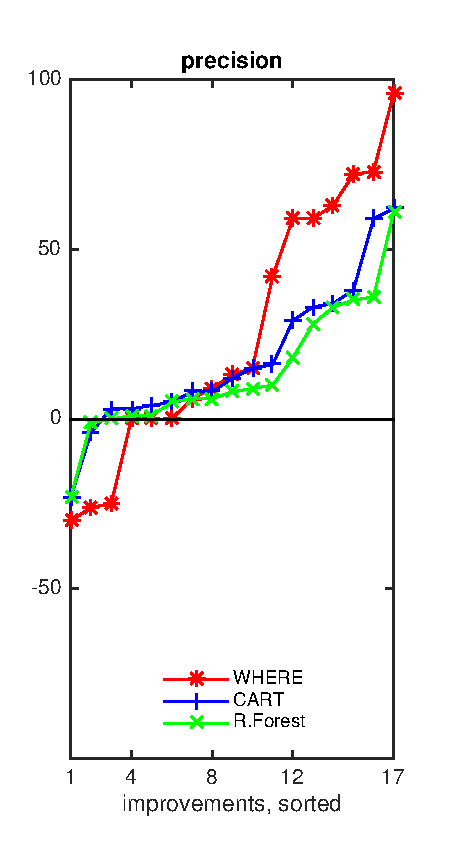
\includegraphics[width=1.5in]{precision_W.eps}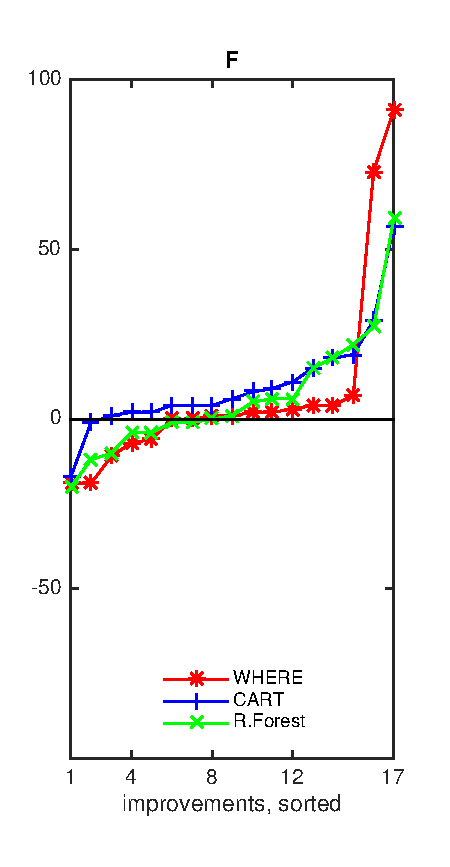
\includegraphics[width=1.5in]{F_W.eps}
 \end{center}
\caption{Deltas in performance  seen in \fig{precisionbars} (left)
and \fig{fbars} (right) between tuned and untuned learners. Tuning improves performance when the deltas are above zero.}\label{fig:deltas}
 \end{figure}

\subsection{RQ2:  Does Tuning Change a Learner's Ranking Regarding Different Goals?}\label{sect:rank}
Researchers often use performance criteria to assert that one learner is better than another~\cite{lessmann2008benchmarking,me07b}. In\cite{me07b}, naive Bayes does better than C4.5 in terms of pd and balance over NASA MDP data sets. In \cite{lessmann2008benchmarking}, Random Forest is considered to be statistically better than CART in terms of the AUC ranking. Such conclusions are not reliable since they can change when we elect to tune for different goals.

22 learners are compared over NASA MDP data sets in terms of the AUC in \cite{lessmann2008benchmarking}. Some learners are tuned using manual methods, like C4.5, CART and Random Forests and some are tuned by searching algorithms, like grid search for SVM-Type learners. In our expeirment, when we tune CART and Random Forests for precisoin and F-measure, the rankings of these two learners are changed.

In \fig{precisionbars} and \fig{fbars}, the tuned CART are better than or equal to tuned Random Forests over $\frac{11}{17}$ and $\frac{10}{17}$ data sets in
terms of precision and F-measure, respectively. Results from the non-parametric Kolmogorov-Smirnov Test turn out that the performance 
scores of tuned CART and tuned Random Forests are not statistically different. This is the pposite of   
 Lessmann et al.~\cite{lessmann2008benchmarking}, the tuned Random Forest is not significantly better than tuned CART.
 In another result that is the reverse of \fig{precisionbars}, tuned WHERE is not necessarily
 any better than anything else.
 
 Therefore, it's not always safe to say ``LearnerX'' is the best or better than ``learnerY'' without pointing out the performance criteria or applying tuning techniques. That is, the answer to RQ2 is ``yes'' since tuning a set of learners
 changes the rankings of those learners regarding different criteria.
 
The  important lesson here is that, given a particular task (e.g. optimizing for precision), tuning can offer
substantial benefits. However, when that task changes (e.g. to optimizing for the F-measure),
it should not be assumed that conclusions from the previous tuning will hold in the new context.
In practice, this means that tuning needs to be repeated for each new context.





\begin{figure}[!t]
\renewcommand{\baselinestretch}{0.8} 

\scriptsize  
~~~\begin{tabular}{r|rl|rl|rl|rl|rl|rlrl}
      &   \multicolumn{4}{c|}{WHERE}         &   \multicolumn{4}{c|}{CART}         &   \multicolumn{4}{c}{Random Forest}         \\\hline
  Data set   &   \multicolumn{2}{c}{default}         &   \multicolumn{2}{c|}{Tuned}         &   \multicolumn{2}{c}{default}         &   \multicolumn{2}{c|}{Tuned}    &   \multicolumn{2}{c}{default}  &   \multicolumn{2}{c}{Tuned}\\\hline
antV0 & 39 &   & 20 &   & 32 &   & 40 &   & {\bf 41} &   & 21 &  \\
antV1 & 11 &   & 5 &   & 38 &   & 49 &   & 37 &   & {\bf 55} &  \\
antV2 & 0 &   & 3 &   & 44 &   & {\bf 48} &   & 47 &   & 46 &  \\
camelV0 & 0 &   & {\bf 91} &   & 9 &   & 28 &   & 4 &   & 31 &  \\
camelV1 & 35 &   & 35 &   & 31 &   & 33 &   & {\bf 37} &   & 33 &  \\
ivy & 28 &   & 32 &   & 28 &   & 30 &   & 27 &   & {\bf 33} &  \\
jeditV0 & 50 &   & {\bf 57} &   & 56 &   & {\bf 57} &   & 56 &   & {\bf 57} &  \\
jeditV1 & 37 &   & 38 &   & 36 &   & 45 &   & 43 &   & {\bf 49} &  \\
jeditV2 & 4 &   & 6 &   & 5 &   & {\bf 9} &   & {\bf 9} &   & 8 &  \\
log4j & {\bf 61} &   & 54 &   & 47 &   & 46 &   & 57 &   & 45 &  \\
lucene & 70 &   & 74 &   & 56 &   & 74 &   & 70 &   & {\bf 75} &  \\
poiV0 & 82 &   & 71 &   & 79 &   & 62 &   & {\bf 83} &   & 73 &  \\
poiV1 & 5 &   & {\bf 78} &   & 21 &   & {\bf 78} &   & 19 &   & {\bf 78} &  \\
synapse & 0 &   & 2 &   & 40 &   & 55 &   & 41 &   & {\bf 56} &  \\
velocity & 51 &   & 51 &   & 49 &   & {\bf 53} &   & 51 &   & 51 &  \\
xercesV0 & 22 &   & 23 &   & 21 &   & {\bf 27} &   & 24 &   & 20 &  \\
xercesV1 & 23 &   & 4 &   & 18 &   & {\bf 47} &   & 18 &   & 40 &  \\
\end{tabular}
\caption{F-value results (best results  shown in {\bf bold}).}
\label{fig:fbars}
\end{figure}


\subsection{RQ3: Does Tuning Select Different Project Factors? }\label{sect:import}


Researchers often use data miners to  test what factors have most impact on software projects~\cite{bell2013limited,rahman2013how,me02k,moser2008comparative,zimmermann2007predicting,herzig2013predicting}. 
\fig{features} shows that such conclusions are not reliable since they can be changed by tuning. For space limitation, from each data set, we just select one experiment, like antV0, as representative. 
This figure shows what attributes appeared in WHERE's final decision trees when optimizing for different goals, precision and F-measure. Note that the attributes selected by tuned WHERE in each row shown in bold are usually different from default WHERE. Meanwhile, Tuning for different goals will usually select different attributes. In $\frac{9}{10}$ representative experiments, tuning select different attributes for precision and F-measure.
% Note that the counts in the {\em tuned} column are   usually
% different to those in the {\em default} columns (the tuned learners used more attributes
% than otherwise as witnessed by the taller columns of numbers in the ``tuned'' column). 

That is, our answer to RQ3 is ``yes'', tuning changes our
conclusions about what factors are most in important in software engineering.




\subsection{RQ4: Is Tuning Easy?}\label{sect:easy}

In terms of the search space
explored via tuning, optimizing defect prediction from static code
measures is much {\em smaller} than the standard optimization.

To see this,
recall from Algorithm~1 that
DE explores a {\em Population} of size {\em np=10}. This is a very small population size since
Rainer Storn (one of the inventors of DE) recommends  setting {\em np} to be ten times larger than the number
of attributes being optimized~\cite{storn1997differential}.

From \fig{parameters},
we see that Storn would therefore recommend {\em np} values of
90, 50, 60 for WHERE, CART and Random Forests (respectively). Yet we achieve our results
using a constant {\em np=10}; i.e. $\frac{10}{90}, \frac{10}{50}, \frac{10}{60}$ of the
recommended search space.

Another measure showing that tuning is easy 
(for static code defect predictors)
is the number of evaluations required to complete optimization
(see next section).

Hence we answer RQ4 as ``yes'', tuning is surprisingly easy (at least
for defect predictors).
% list some features
\begin{figure*}[!ht]

\renewcommand{\baselinestretch}{0.8}
\scriptsize
\centering
  \begin{tabular}{c|l|l}
    \multicolumn{1}{c|}{ Data set}  &   \multicolumn{1}{c|}{Precision} & \multicolumn{1}{c}{F} \\ \hline
  \multirow{2}{*}{antV0} & {\bf mfa} &  {\bf None} \\
         & mfa, dam, wmc, ic & mfa, dam, wmc, ic\\
  \hline
 \multirow{2}{*}{camelV0} & {\bf mfa, rfc, lcom3, cam, amc, loc, ic} &{\bf  mfa, wmc, cam, dam, loc, lcom3, rfc, ic, dit }\\
        & mfa, rfc, lcom3, cam, dam, loc & mfa, rfc, lcom3, cam, dam, loc\\
  \hline
 \multirow{2}{*}{ivy} & {\bf dam, cam} &{\bf  cam, dit, npm, dam, wmc, lcom3 }  \\
       & cam, dit, dam, ic & cam, dit, dam, ic \\
  \hline
 \multirow{2}{*}{jeditV0} &{\bf  mfa, dam, rfc, avg\_cc, lcom3, dit }&{\bf  dam, rfc, mfa, wmc, ce, cam, loc, avg\_cc}\\
         & mfa, dam, lcom3, dit, ic, cbm & mfa, dam, lcom3, dit, ic, cbm \\
  \hline
 \multirow{2}{*}{log4j} & {\bf lcom3, mfa, loc, cbm, wmc }&{\bf  mfa, wmc}\\
         & lcom3, mfa, loc, cbm, dit & lcom3, mfa, loc, ic \\
   \hline
  \multirow{2}{*}{lucene} & {\bf rfc, mfa, npm, cam} & {\bf mfa, dam, wmc, loc, rfc, ic}\\
         & mfa, lcom3, cam, dam, ic & mfa, lcom3, cam, dam, ic\\
   \hline
   \multirow{2}{*}{poiV0} & {\bf loc }& {\bf loc} \\
        & mfa, loc, amc, wmc, npm, lcom & mfa, loc, amc, wmc,npm, lcom\\
   \hline
   \multirow{2}{*}{synapse} &{\bf  dam} & {\bf loc, dam} \\
        & dam, loc, mfa, cam & dam, loc, mfa, cam\\
    \hline
   \multirow{2}{*}{velocity} & {\bf dit, dam, cam, rfc, cbo, lcom3, wmc, ic, cbm }& {\bf dam, dit, loc, amc, lcom3, ic, mfa }\\
        & dit, dam, lcom3, ic, mfa  & dit, dam, lcom3, ic, mfa\\
    \hline
   \multirow{2}{*}{xercesV0} &{\bf  None }&{\bf  dam, rfc, avg\_cc, dit, loc, lcom3, cam }\\
        & cam, loc, dam, mfa, amc &  cam, loc, dam, mfa, amc \\
    \hline
    
  \end{tabular}
  
    \caption{Features selected by different goals(features selected by tuning shown in bold). 
    }\label{fig:features}
\end{figure*}




\begin{figure}[!ht]

\renewcommand{\baselinestretch}{0.8}
\scriptsize
\centering
  \begin{tabular}{c|c c|c c|c c|c c| c c }
  
    &   \multicolumn{2}{c|}{Precision} & \multicolumn{2}{c|}{F} &  \multicolumn{2}{c|}{SUM}\\
 &&&&&&&\\
Features&   
  default
& tuned
& default
& tuned
& default
& tuned
\\\hline

max\_cc& & & &  & & \\
noc& & & & & & \\
ca& & & & & & \\
cbo& & 1& & & & 1\\
moa& & 1& & & & 1\\
ce& & 2& & 1& & 3\\
avg\_cc& & 2& & 2& & 4\\
npm& 1& 2& 1& 1&2 & 3\\
lcom& 1& 2& 1& 1& 2& 3\\
amc& 4& 2& 4& 2& 8& 4\\
cbm& 5& 2& 5& 3& 10& 5\\
rfc& 3& 6& 3& 8& 6& 14\\
wmc& 5& 4& 5& 9& 10& 13\\
dit& 8& 3& 7& 7& 15& 10\\
ic& 8& 3& 8& 6& 16 & 9\\
lcom3& 8& 6& 8& 8&16 & 14\\
cam& 9& 7& 9& 7& 18& 14\\
loc& 9& 5& 9& 11& 18& 16\\
dam& 13& 6& 13& 11& 26& 17 \\
mfa& 16& 9& 16& 9&32 & 18\\

 
  \end{tabular}
    \caption{Counts of features selected by different goals.Given that we are processing 17 data sets, the maximum counts for any 
one cell in the ``precision'' or ``F'' column is 17.  
    }\label{fig:counts}
\end{figure}
 

\begin{figure*}[!ht]

\renewcommand{\baselinestretch}{0.75}
\scriptsize
\centering
  \begin{tabular}{r|c |c |c |c |c |c }
    Datasets & Tuned\_Where & Default\_Where & Tuned\_CART & Default\_CART & Tuned\_RanFst & Default\_RanFst\\
    \hline
    antV0 & 50 / 90.18 & 1.57 & 60 / 4.36 & 0.09 & 50 / 8.12 & 0.18\\
    antV1 & 50 / 174.67 & 2.90 & 50 / 6.35 & 0.10 & 50 / 11.77 & 0.27\\
    antV2 & 50 / 403.63 & 6.92 & 70 / 9.71 & 0.16 & 60 / 13.28 & 0.35\\
    camelV0 & 50 / 537.53 & 8.60 & 50 / 9.14 & 0.18 & 50 / 13.73 & 0.31\\
    camelV1 & 60 / 1640.54 & 24.57 & 60 / 17.06 & 0.24 & 70 / 31.53 & 0.73\\
    ivy & 70 / 77.75 & 1.02 & 60 / 3.86 & 0.06 & 50 / 8.00 & 0.17\\
    jeditV0 & 80 / 472.57 & 5.49 & 60 / 6.30 & 0.09 & 70 / 13.01 & 0.30\\
    jeditV1 & 60 / 489.45 & 6.82 & 70 / 7.61 & 0.11 & 60 / 12.87 & 0.32\\
    jeditV2 & 50 / 435.43 & 7.21 & 50 / 6.46 & 0.12 & 90 / 20.34 & 0.37\\
    log4j & 70 / 113.73 & 1.36 & 70 / 3.25 & 0.05 & 60 / 7.07 & 0.16\\
    lucene & 70 / 224.39 & 2.70 & 50 / 4.07 & 0.08 & 50 / 8.87 & 0.26\\
    poiV0 & 60 / 261.06 & 4.00 & 60 / 6.23 & 0.10 & 50 / 10.57 & 0.29\\
    poiV1 & 80 / 607.85 & 7.18 & 60 / 7.69 & 0.13 & 50 / 11.39 & 0.29\\
    synapse & 50 / 116.04 & 1.87 & 60 / 4.07 & 0.05 & 70 / 9.74 & 0.16\\
    velocity & 60 / 195.27 & 2.75 & 60 / 4.49 & 0.06 & 80 / 12.15 & 0.21\\
    xercesV0 & 60 / 143.69 & 2.17 & 70 / 7.26 & 0.09 & 60 / 10.28 & 0.23\\
    xercesV1 & 50 / 794.50 & 13.37 & 50 / 8.24 & 0.15 & 60 / 14.54 & 0.38\\

  \end{tabular}
  \caption{Evaluations/runtimes  (in seconds), optimizing for  precision.  }\label{fig:etimes}
\end{figure*}
%%%%time for F %%%%%%
\begin{figure*}[!ht]
\renewcommand{\baselinestretch}{0.75}
\scriptsize
\centering
  \begin{tabular}{r|c |c |c |c |c |c } 
    Datasets & Tuned\_Where & Default\_Where & Tuned\_CART & Default\_CART & Tuned\_RanFst & Default\_RanFst\\
    \hline
    antV0 & 50 / 94.08 & 1.71 & 60 / 4.55 & 0.08 & 60 / 10.79 & 0.21\\
    antV1 & 60 / 193.74 & 3.02 & 70 / 7.77 & 0.09 & 60 / 12.30 & 0.25\\
    antV2 & 80 / 643.94 & 7.59 & 60 / 8.38 & 0.15 & 70 / 16.99 & 0.41\\
    camelV0 & 60 / 662.56 & 9.97 & 60 / 13.19 & 0.23 & 80 / 26.11 & 0.32\\
    camelV1 & 60 / 1800.64 & 24.25 & 50 / 15.02 & 0.28 & 50 / 28.52 & 0.78\\
    ivy & 60 / 69.95 & 1.03 & 50 / 3.35 & 0.08 & 70 / 9.40 & 0.18\\
    jeditV0 & 90 / 553.80 & 5.58 & 50 / 5.58 & 0.09 & 60 / 15.08 & 0.33\\
    jeditV1 & 60 / 519.75 & 8.76 & 50 / 7.43 & 0.13 & 60 / 18.13 & 0.41\\
    jeditV2 & 70 / 621.32 & 8.98 & 50 / 9.71 & 0.15 & 60 / 17.38 & 0.63\\
    log4j & 70 / 125.29 & 1.73 & 50 / 2.90 & 0.06 & 60 / 8.76 & 0.19\\
    lucene & 50 / 221.99 & 3.52 & 50 / 5.20 & 0.10 & 50 / 10.09 & 0.33\\
    poiV0 & 60 / 327.48 & 5.13 & 50 / 6.56 & 0.11 & 50 / 12.88 & 0.36\\
    poiV1 & 50 / 523.85 & 8.95 & 80 / 12.26 & 0.14 & 60 / 19.56 & 0.35\\
    synapse & 70 / 148.23 & 1.91 & 60 / 3.96 & 0.06 & 60 / 8.19 & 0.16\\
    velocity & 50 / 156.51 & 2.75 & 60 / 4.27 & 0.06 & 50 / 7.70 & 0.22\\
    xercesV0 & 60 / 142.83 & 2.01 & 70 / 7.15 & 0.08 & 60 / 9.61 & 0.20\\
    xercesV1 & 50 / 751.92 & 12.98 & 60 / 9.28 & 0.16 & 50 / 12.69 & 0.38\\

  \end{tabular}
  \caption{Evaluations/runtimes  (in seconds), optimizing for  ``F''.  }\label{fig:ftimes}
\end{figure*}



\subsection{RQ5: Is Tuning Impractically Slow?}\label{sect:fast}
 
 
The number of evaluations/runtimes used by our optimizers is shown in \fig{etimes}
and \fig{ftimes}.
WHERE's runtimes are slower than CART and Random Forest since WHERE has yet to benefit from decades
of implementation experience with these older algorithms. For example, SciKitLearn's  CART and Random Forest
 make extensive use of an underlying ``C'' library whereas WHERE is a purely interpreted Python.

Looking over \fig{etimes} and \fig{ftimes}, the general pattern is that 50 to 80 evaluations suffice for finding the tuning
improvements reported in this paper. 
50 to 80 evaluations is  much less than our pre-experimental intuition.
Prior to this paper, the authors have conducted numerous explorations of evolutionary algorithms
for search-based SE applications~\cite{krall15,krall15:hm,fea02a,me07f,Green}. Based
on that work, our expectations were that non-parametric evolutionary optimization would
take thousands, if not millions, of evaluations of candidate tunings. Hence, originally,
we used Storn's advise on the size of {\em np} and ran our optimizers for 24 hours. 
Then, just
to get a baseline, we tried {\em np=10} and the early stopping rules (number of lives used in
Algorithm~1 on line 5) and obtained the results of this paper.

Hence, we answer RQ5 as ``no''. Tuning is so fast that
it could (and should) be used by anyone using defect predictors.

\subsection{RQ6: Should we use ``off-the-shelf'' Tunings?}\label{sect:variance}
 
 \fig{preselect} and \fig{fselect} show   tunings learned by DE. 
The left hand side columns shows some standard default values. Note that:
\bi
\item
The tunings learned by DE
were often very different to the default. That is, to achieve the performance improvements seen in the paper,
the default tuning parameters required a wide range of adjustments.
\item The tunings learned by DE were different in different data sets and for different goals. Hence, we answer RQ6 as ``no'' since, to achieve the improvements seen in this paper, tuning has to be repeated whenever the goals or data
sets are changed.
\ei
Given this requirement to repeatedly run tuning, it is fortunate that (as shown above)
tuning is so easy and so fast (at least for defect predictors from static code attributes).




 
%%%%parameters for prec %%%%%%
\begin{figure*}[!ht]
 
\renewcommand{\baselinestretch}{0.9}
\resizebox{\textwidth}{!}{
\scriptsize
\centering
  \begin{tabular}{|c |c |c |c |c |c |c |c |c |c |c |c |c |c |c |c |c |c |c |c |}
    \hline
  \begin{tabular}[c]{@{}c@{}}Learner \\ Name\end{tabular}&Parameters  & Default &antV0&antV1&antV2&camelV0&camelV1&ivy&jeditV0&jeditV1&jeditV2&log4j&lucene&poiV0&poiV1&synapse&velocity&xercesV0&xercesV1\\ 
 \hline
\multirow{8}{*}{\begin{tabular}[c]{@{}c@{}}Where\\based\\ Learner\end{tabular}}
& threshold& 0.5& 0.98& 0.98& 0.43& 0.24& 0.64& 1& 1& 0.98& 0.98& 1& 1& 0.87& 0.59& 0.98& 1& 0.98& 0.98\\ \cline{2-20}
& infoPrune& 0.33& 0.05& 0.05& 0.71& 0.54& 0.45& 0.41& 0.3& 0.05& 0.05& 0.54& 0.84& 0.01& 1& 0.05& 0.68& 0.43& 0.05\\ \cline{2-20}
& min\_sample\_size& 4& 7& 7& 9& 8& 6& 10& 1& 5& 7& 8& 7& 9& 3& 7& 7& 1& 7\\ \cline{2-20}
& min\_Size& 0.5& 0.51& 0.51& 0.59& 0.46& 0.13& 0.38& 0.66& 0.27& 0.51& 0.46& 0.47& 0.77& 0.48& 0.51& 0.66& 0.22& 0.51\\ \cline{2-20}
& wriggle& 0.2& 0.6& 0.6& 0.83& 0.52& 0.19& 0.01& 0.26& 0.6& 0.6& 0.52& 0.19& 0.83& 0.01& 0.6& 0.26& 0.55& 0.6\\ \cline{2-20}
& depthMin& 2& 1& 1& 2& 3& 5& 2& 3& 3& 1& 1& 2& 4& 2& 1& 3& 2& 1\\ \cline{2-20}
& depthMax& 10& 8& 8& 13& 19& 19& 18& 7& 8& 8& 19& 1& 19& 18& 8& 11& 18& 8\\ \cline{2-20}
& wherePrune& False& False& False& False& False& True& True& False& False& False& False& False& True& True& False& False& True& False\\ \cline{2-20}
& treePrune& True& False& False& False& True& True& True& False& False& False& True& True& False& False& False& False& True& False\\ \cline{2-20}
\hline
\multirow{4}{*}{CART}
& threshold& 0.5& 0.69& 0.99& 1& 0.3& 0.83& 1& 0.99& 0.58& 0.72& 1& 0.71& 0.46& 0.72& 1& 0.85& 1& 0.64\\ \cline{2-20}
& max\_feature& None& 0.01& 0.58& 0.65& 0.66& 0.73& 0.67& 0.56& 0.01& 0.97& 0.54& 0.52& 0.32& 0.01& 0.74& 0.73& 0.01& 0.1\\ \cline{2-20}
& min\_samples\_split& 2& 7& 16& 18& 5& 11& 6& 15& 6& 17& 4& 16& 12& 5& 14& 11& 4& 10\\ \cline{2-20}
& min\_samples\_leaf& 1& 13& 14& 10& 4& 3& 15& 16& 9& 6& 7& 6& 1& 4& 6& 7& 11& 7\\ \cline{2-20}
& max\_depth& None& 14& 1& 41& 34& 1& 22& 29& 1& 1& 1& 14& 19& 8& 40& 4& 1& 1\\ \cline{2-20}
\hline
\multirow{6}{*}{\begin{tabular}[c]{@{}c@{}}Random \\ Forests\end{tabular}} 
& threshold& 0.5& 0.84& 0.9& 0.83& 0.33& 1& 0.99& 0.91& 1& 1& 0.83& 0.98& 0.9& 0.86& 0.83& 1& 1& 1\\ \cline{2-20}
& max\_feature& None& 0.61& 0.13& 0.89& 0.37& 0.01& 0.98& 0.52& 0.75& 0.35& 0.01& 0.98& 0.84& 0.73& 0.01& 0.48& 0.51& 0.01\\ \cline{2-20}
& max\_leaf\_nodes& None& 37& 35& 38& 21& 36& 45& 10& 38& 10& 30& 20& 43& 11& 13& 15& 39& 10\\ \cline{2-20}
& min\_samples\_split& 2& 8& 16& 17& 13& 14& 2& 3& 2& 2& 18& 19& 9& 4& 4& 9& 20& 1\\ \cline{2-20}
& min\_samples\_leaf& 1& 19& 5& 2& 4& 2& 4& 7& 17& 7& 16& 12& 2& 3& 2& 2& 2& 3\\ \cline{2-20}
& n\_estimators& 100& 138& 112& 77& 74& 125& 130& 107& 85& 96& 111& 103& 82& 59& 149& 150& 63& 58\\ \cline{2-20}
\hline  \end{tabular}
}
  \caption{Parameters tuned on different models over the objective of precision.}\label{fig:preselect}
\end{figure*}


%%%%parameters for F %%%%%%
\begin{figure*}[!ht]
 
\resizebox{\textwidth}{!}{
\renewcommand{\baselinestretch}{0.9}
\scriptsize
\centering
  \begin{tabular}{|c |c |c |c |c |c |c |c |c |c |c |c |c |c |c |c |c |c |c |c |}
    \hline
    
  \begin{tabular}[c]{@{}c@{}}Learner \\ Name\end{tabular}&Parameters  & Default &antV0&antV1&antV2&camelV0&camelV1&ivy&jeditV0&jeditV1&jeditV2&log4j&lucene&poiV0&poiV1&synapse&velocity&xercesV0&xercesV1\\ 
 \hline
\multirow{8}{*}{\begin{tabular}[c]{@{}c@{}}Where\\based\\ Learner\end{tabular}}
& threshold& 0.5& 0.04& 0.44& 0.44& 0.98& 0.65& 0.77& 1& 0.65& 0.98& 0.44& 0.44& 0.87& 0.04& 0.77& 0.24& 0.44& 0.77\\ \cline{2-20}
& infoPrune& 0.33& 0.51& 0.68& 0.88& 0.47& 0.07& 0.31& 0.48& 0.68& 0.57& 0.12& 0.68& 0.01& 0.51& 0.14& 0.54& 0.68& 0.14\\ \cline{2-20}
& min\_sample\_size& 4& 6& 4& 6& 1& 6& 8& 8& 4& 6& 7& 4& 9& 6& 2& 8& 4& 8\\ \cline{2-20}
& min\_Size& 0.5& 0.18& 0.4& 0.56& 0.51& 0.65& 0.59& 0.97& 0.4& 0.51& 0.8& 0.4& 0.77& 0.18& 0.62& 0.46& 0.4& 0.66\\ \cline{2-20}
& wriggle& 0.2& 0.25& 0.29& 0.76& 0.6& 0.63& 0.26& 1& 0.51& 0.17& 0.36& 0.51& 0.83& 0.25& 0.5& 0.52& 0.29& 0.26\\ \cline{2-20}
& depthMin& 2& 3& 3& 3& 1& 5& 3& 2& 3& 5& 5& 3& 4& 3& 3& 3& 3& 3\\ \cline{2-20}
& depthMax& 10& 16& 15& 15& 8& 19& 10& 7& 15& 5& 15& 15& 19& 16& 6& 19& 15& 10\\ \cline{2-20}
& wherePrune& False& False& True& True& True& True& True& True& False& False& True& True& True& False& True& False& False& True\\ \cline{2-20}
& treePrune& True& False& True& True& False& False& False& False& False& True& True& True& False& False& False& True& True& False\\ \cline{2-20}
\hline
\multirow{5}{*}{CART}
& threshold& 0.5& 0.34& 0.25& 0.01& 0.01& 0.73& 0.53& 0.92& 0.8& 0.74& 0.54& 0.03& 0.91& 0.01& 0.01& 0.55& 1& 0.01\\ \cline{2-20}
& max\_feature& None& 0.01& 0.01& 0.29& 0.01& 0.46& 0.75& 0.79& 0.74& 0.41& 0.81& 0.61& 0.72& 0.01& 0.01& 0.01& 0.25& 0.18\\ \cline{2-20}
& min\_samples\_split& 2& 18& 20& 12& 2& 15& 11& 2& 18& 13& 9& 17& 16& 10& 4& 8& 3& 15\\ \cline{2-20}
& min\_samples\_leaf& 1& 19& 16& 15& 17& 1& 1& 13& 10& 4& 3& 7& 5& 20& 7& 8& 1& 6\\ \cline{2-20}
& max\_depth& None& 12& 2& 15& 1& 41& 20& 44& 15& 13& 5& 23& 14& 1& 5& 17& 47& 13\\ \cline{2-20}
\hline
\multirow{6}{*}{\begin{tabular}[c]{@{}c@{}}Random \\ Forests\end{tabular}} 
& threshold& 0.5& 0.01& 0.35& 0.3& 0.01& 0.9& 0.97& 0.63& 1& 0.73& 0.68& 0.01& 1.0& 0.01& 0.07& 0.22& 1& 0.82\\ \cline{2-20}
& max\_feature& None& 0.63& 0.17& 0.01& 0.01& 0.88& 0.74& 0.76& 0.73& 0.01& 0.03& 0.39& 0.02& 0.01& 0.56& 0.36& 0.51& 0.89\\ \cline{2-20}
& max\_leaf\_nodes& None& 40& 33& 46& 22& 11& 16& 38& 34& 30& 31& 12& 49& 25& 47& 15& 39& 24\\ \cline{2-20}
& min\_samples\_split& 2& 10& 16& 20& 1& 1& 1& 1& 4& 20& 19& 11& 14& 2& 17& 19& 20& 19\\ \cline{2-20}
& min\_samples\_leaf& 1& 4& 15& 9& 13& 18& 11& 3& 16& 17& 6& 10& 7& 19& 13& 11& 2& 14\\ \cline{2-20}
& n\_estimators& 100& 120& 73& 75& 130& 97& 144& 125& 97& 80& 111& 96& 101& 50& 67& 74& 63& 66\\ \cline{2-20}
\hline  \end{tabular}
}
  \caption{Parameters tuned on different models over the objective of ``F''.}\label{fig:fselect}
\end{figure*}


\section{Reliability and Validity}\label{sect:construct}


{\em Reliability} refers to the consistency of the results obtained
from the research.  For example,   how well independent researchers
could reproduce the study? To increase external
reliability, this paper has taken care to either  clearly define our
algorithms or use implementations from the public domain
(SciKitLearn). Also, all the data used in this work is available
on-line in the PROMISE code repository and all our algorithms
are on-line at github.com/a-se/where.


{\em Validity} refers to the extent to which a piece of research actually
investigates what the researcher purports to investigate.
{\em Internal validity} checks if the differences found in
the treatments can be ascribed to the treatments under study. 
One internal validity issue with our experiments is the choice
of {\em training, tuning, and testing} data sets discussed in 
\tion{design}. Recall that while all our learners used the same
{\em testing} data set, our untuned learners were only given
access to {\em training} while DEs could get feedback from
{\em training} and
{\em tuning}.  This mean that, potentially,  the performance increases
reported above are merely an artificat of the DEs being able to access
more data. However:
\bi
\item Note that
DEs assess their performance using a model built from {\em training}
then applied to the {\em tuning} data. If we gave the untuned
learners double the training data, then this would be inherently
biased against DEs.
\item In practice, this is much ado about nothing. We have
repeated all the experiments of this paper with the untuned
learners building models from {\em training} + {\em tuning}.
While the exact numbers found in this way
may differ from the above in some small way, we can report that 
those repeated runs do not substantively change the above conclusions.
\ei
{\em External validity} checks if the results are of relevance
for other cases, or can be generalized from samples
to populations.  
The examples of this paper  only relate to precision, recall, and the F-measure
but the general principle (that the search bias changes the search conclusions)  holds for all any set of goals. 
Also,
the tuning results shown here only came from one  software analytics task 
(defect prediction from static code attributes).
There are many other kinds of software analytics tasks 
(software development effort estimation, social network mining,
detecting duplicate issue reports, etc) and the implication of this
study for those tasks is unclear. 
However,  those other tasks often use the same kinds of learners
explored in this paper so it is quite possible that
the conclusions of this paper apply to other SE analytics tasks as well. 

That said, there exist some class of data mining papers for which
tuning may not be required. Consider  Le Goues et al.'s 2012
ICSE paper that used a evolutionary program to learn
repairs to code~\cite{leGoues12}. The performance criteria
in that paper was ``can we fix any of the known bugs?''. Note
that this criteria is a ``{\em competency}'' statement, and
not a ``{\em better than}'' statement (the difference being that
one is 
``can do'' and the other is ``can do better''). For such
competency claims, tuning is not necessary. However, as soon
as {\em better than} enters the performance criteria then this
becomes a race between competing methods. In such a race,
it is unfair to hobble one competitor with poor tunings.



\section{Conclusions}

Our exploration of the six research
questions listed in the introduction
show that when learning defect predictors for static code
attributes,   analytics without parameter tuning is considered {\em harmful} and {\em misleading}:
\bi
\item Tuning improves the performance scores of a predictor.
That improvement is usually positive (see \fig{deltas}) and sometimes
it can be quite   dramatic (e.g. precision changing from 2\% to 98\%). \item 
Tuning changes conclusions on what learners are better than others.
Hence, it is time to revisit numerous prior publications of our own~\cite{me07b}
and others~\cite{lessmann2008benchmarking,hall11}.
\item
Also,
tuning changes  changes conclusions on what factors are most important in software development.
Once again, this means that old papers may need to be revised including those
some of our own~\cite{me02k} and others~\cite{bell2013limited,rahman2013how,moser2008comparative,zimmermann2007predicting,herzig2013predicting}. 
\ei
Accordingly, we strongly advise that data miners should not be used ``off-the-shelf'' with their default tunings. 
\fig{preselect} and \fig{fselect}    show just how much tuning can alter default settings
both for different data sets and for different goals. 

Since the results from tuning are unstable,
tuning needs to be repeated
whenever data or goals are changed.
Fortunately, the cost of find good tunings is not excessive since, at least for
static code defect predictors, tuning is easy and fast.

\section{Future Work}

 As noted by
F\"{u}rnkranz~\cite{furnkranz05}, data mining is inherently a multi-objective optimization
problem that seeks the smallest model with the highest performance, 
that generalizes best for
future examples (perhaps learned in minimal time using the least amount of data).
In this view, we are using DE to optimize an optimizer. Perhaps a better approach might be
to dispense with the separation of ``optimizer'' and ``learner'' and combine them both
into one system that learns how to tune itself as it executes. If this view is useful,
then instead of adding elaborations to data miners (as done in this paper, or by researchers
exploring hyper-heuristics~\cite{jia2013learning}), it should be possible to radically simplify optimization and data
mining with a single system that rapidly performs both tasks.

Another issue for future work is the implications of these
conclusions to other kinds of software analytics.
 This paper has explored  {\em some} learners using {\em one}  optimizer. Hence, we can make
no claim that DE is the {\em best} optimizer for {\em all} learners.
Rather, our point is that there exists at least some learners
whose performance can be dramatically improved by 
at least one simple optimization scheme.  We hope that this work inspires
much future work as this community develops and debugs best practices for tuning
software analytics.
 
 

\section*{Acknowledgments}
The work has partially funded by a National Science Foundation CISE CCF award \#1506586.
 
\vspace*{0.5mm}
 
 
\bibliographystyle{plain}

\balance
\bibliography{tuningpredictor}  

   



  


  

\end{document}
 
\subsection{Implications}

time for an end to era of data mining in se? moving on to a new phase of learning-as-optimization

1) learning is actually an optimization tasks (e.g. see fig2 of  learners climbing the roc curve hill in http://goo.gl/x2EaAm)

2) our learners are all contorted to do some tasks X (e.g. minimize expected value of entropy), then we assess them on score Y (recall). which is nuts. maybe we should build the goal predicate into the learner (e.g http://menzies.us/pdf/10which.pdf) 

3) given 1 + 2, maybe the whole paradigm of optimizing param selection is wrong. maybe what we need is a library of bees buzzing around making random choices (e.g. about descritziation) which other bees use, plus their own random choices (e.g. max depth of tree learned from discretized data) which is used by other bees, plus their own random choices (e.g. business users reading the models).  the funky thing here is that it can take some time before some of the bees (the discretizers) get feedback from the community of people using their decision (the tree learners). 




